\section{Cheeger不等式}
\label{sec:graph-cheeger}

前一节用组合拉普拉斯的第二小特征值$\lambda_2$衡量图连得有多紧。但$\lambda_2$会随边权的整体放大而增大，两张规模不同的图之间直接比较$\lambda_2$并不公平。

一种更合理的衡量方式是：割掉一组边后，组间断开的边权占较小一侧总连接量的多少？如果一座大桥连接两个城市群，桥虽然只有一条，但两侧各自有大量内部道路，切断这一条边对较小一侧的影响取决于那一侧总共有多少路。相比之下，切下一个只有一条边的孤立叶子，割权同为一，但那个叶子的全部连接就是这一条边。

以下假定正权支撑连通，这保证每个顶点都有正度。

\subsection{导通率}
\label{sec:graph-conductance}

用$S$和$\bar S=V\setminus S$表示一组顶点和剩下的顶点，要求两组都非空。把一端在$S$、另一端在$\bar S$的边各数一次，将它们的权重相加，得到\term{割权}（cut weight）$c(S,\bar S)$。

顶点$i$的加权度$d_i$是连到该点的所有边权之和。将$S$内每个点的度累加，得到集合体积$\operatorname{vol}(S)=\sum_{i\in S}d_i$。体积的计算中，组内边在两个端点各被计入一次，跨边只在组内的那个端点计入。图~\ref{fig:graph-conductance-volume}标出了这两种计数。

\begin{BookInlineFigure}
  \centering
  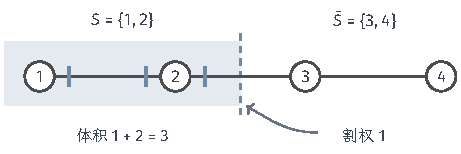
\includegraphics{figures/03-graphs/05-matrices-and-spectra/tikz/conductance-volume/figure.pdf}
  \caption{单位权四点路径上$S=\{1,2\}$的体积计算。每道刻度表示一个边端点处计入的一份。边$12$两端都在$S$中，计两份；边$23$只有一端在$S$中，计一份。左侧体积为$3$。虚线切过的边只有$23$，割权为$1$。}
  \label{fig:graph-conductance-volume}
\end{BookInlineFigure}

用体积较小的一侧来衡量规模。分母越小，同样的割权所占的比例就越大。

\begin{definition}[导通率]
\label{def:graph-conductance}
集合的\term{导通率}（conductance）和图的最小导通率分别为
\begin{equation}
\label{eq:graph-conductance}
\phi(S)=\frac{c(S,\bar S)}
  {\min\{\operatorname{vol}(S),\operatorname{vol}(\bar S)\}},
\qquad
\phi_*=\min_{\varnothing\ne S\subsetneq V}\phi(S).
\end{equation}
\end{definition}

在单位权四点路径上试两种切法。把中间边$23$切断，得到$\{1,2\}$和$\{3,4\}$。顶点$1$的度为$1$，顶点$2$的度为$2$，左侧体积为$1+2=3$。右侧的度分别为$2,1$，体积也为$3$。跨边只有一条，割权为$1$，所以这个割的导通率为$1/3$。

如果只切下端点$1$，割权仍为$1$，但$\{1\}$的体积只有$1$，另一侧体积为$5$。导通率变成$1/1=1$。

两种割的割权相同，但中间割的较小一侧承载了更多连接（体积$3$对$1$），所以按比例算，中间割更"高效"。在所有切法中选最小的导通率，就是图的$\phi_*$。

接下来要用归一化拉普拉斯的第二小特征值$\mu_2$来控制$\phi_*$。回顾第~\ref{sec:graph-normalized-laplacian}节，对称归一化拉普拉斯$\mathcal L=\bm D^{-1/2}\bm L\bm D^{-1/2}$的变分刻画为
\begin{equation}
\label{eq:graph-normalized-variational-cut}
\mu_2=\min_{\substack{\bm f^\top\bm D\bm1=0\\\bm f\ne\bm0}}
       \frac{\bm f^\top\bm L\bm f}{\bm f^\top\bm D\bm f}.
\end{equation}
这里的分母把每个坐标的平方乘以该点的度再求和，而不是简单的平方和。零方向对应的条件也变成度加权的零和$\sum_i d_i f_i=0$。若将$S$内的坐标设为$1$，其余设为$0$，分母恰好是$\operatorname{vol}(S)$。因此体积与归一化谱之间有了直接联系。

\begin{theorem}[\term{Cheeger不等式}]
\label{thm:graph-cheeger}
有限无向非负权图的正权支撑连通，且至少有两个顶点时，
\begin{equation}
\label{eq:graph-cheeger}
\frac{\mu_2}{2}\leq\phi_*\leq \sqrt{2\mu_2}.
\end{equation}
\end{theorem}

两个界各回答一个问题。下界说：无论怎样选择分组，其导通率都至少为$\mu_2/2$，图中不存在比这更稀疏的平衡割。上界则提供了一种构造性的搜索：按第二特征方向的分量给顶点排序，依次尝试切点，其中至少有一个割的导通率不超过$\sqrt{2\mu_2}$。

下面分别证明这两个界。

\subsection{下界：指示向量的Rayleigh商}
\label{sec:graph-cheeger-lower}

为证明下界，我们从任意一个割出发，构造一个满足约束的试探向量，再把它代入式~\eqref{eq:graph-normalized-variational-cut}。

取任意非空真子集$S$，设$a=\operatorname{vol}(S)\leq\operatorname{vol}(\bar S)=b$。从$S$的指示向量$\bm 1_S$出发，把每个坐标减去度加权平均值$a/(a+b)$，得到
\[
\bm f=\bm1_S-\frac{a}{a+b}\bm1.
\]
$\bm f$在$S$上取值$b/(a+b)$，在$\bar S$上取值$-a/(a+b)$。度加权的坐标和为
\[
a\cdot\frac{b}{a+b}+b\cdot\frac{-a}{a+b}=0,
\]
满足零和条件$\bm f^\top\bm D\bm 1=0$。

下面分别计算分子和分母。对组内的一条边，两端取同一个值，差为零，不贡献能量。对跨边，两端分别取$b/(a+b)$和$-a/(a+b)$，差恰好为$1$。因此分子等于割权：
\[
\bm f^\top\bm L\bm f=c(S,\bar S).
\]

分母将两侧的常数平方各按体积累加：
\[
\bm f^\top\bm D\bm f
=a\left(\frac{b}{a+b}\right)^{\!2}
+b\left(\frac{a}{a+b}\right)^{\!2}
=\frac{ab}{a+b}.
\]

$\mu_2$是所有合格向量中Rayleigh商的最小值。把$\bm f$代入，给出上界
\[
\mu_2
\leq\frac{c(S,\bar S)}{\dfrac{ab}{a+b}}
=c(S,\bar S)\left(\frac{1}{a}+\frac{1}{b}\right).
\]
因为$a\leq b$，有$1/b\leq 1/a$，所以
\[
\frac{1}{a}+\frac{1}{b}\leq\frac{2}{a}
=\frac{2}{\min\{\operatorname{vol}(S),\operatorname{vol}(\bar S)\}}.
\]
代入得$\mu_2\leq 2\phi(S)$。这个结论对每个非空真子集$S$都成立，因此对所有割取最小后，$\mu_2/2\leq\phi_*$。

用四点路径的中间割核对。两侧体积$a=b=3$，中心化后两侧的坐标分别为$1/2$和$-1/2$。只有一条跨边，割权为$1$。分母为$3\cdot(1/2)^2+3\cdot(1/2)^2=3/2$。代入得$\mu_2\leq 1/(3/2)=2/3$，恰好是$2\phi(S)=2\cdot(1/3)$。

\subsection{上界：扫描阈值}
\label{sec:graph-cheeger-sweep}

下界告诉我们导通率不可能太小。上界则要找到一个具体的割来展示它也不会太大。思路是从归一化拉普拉斯的第二特征方向出发，对顶点排序后逐个阈值切开，证明其中至少有一个割的导通率不超过$\sqrt{2\mu_2}$。

证明分三步。第一步从特征方向中选出一侧体积不超过半图的非负向量。第二步用积分论证，说明沿该向量的阈值扫描中，导通率的加权平均可以用能量商控制。第三步用Cauchy--Schwarz不等式把能量商和$\mu_2$联系起来。

\paragraph{第一步：选出合适的一侧}

设$\bm f$是式~\eqref{eq:graph-normalized-variational-cut}的一个最优向量，能量商恰为$\mu_2$。按分量从小到大排列各顶点，逐个累计加权度。累计首次达到$\operatorname{vol}(V)/2$时，取该顶点的分量值作为度加权中位数$\tau$。严格小于$\tau$的顶点体积不超过半图，严格大于$\tau$的也不超过半图。

将$\bm f$平移为$\bm h=\bm f-\tau\bm 1$。平移对每条边的差没有影响，所以能量$\bm h^\top\bm L\bm h=\bm f^\top\bm L\bm f$不变。对于度加权平方和，展开得到
\[
\bm h^\top\bm D\bm h
=\bm f^\top\bm D\bm f
-2\tau\underbrace{\bm f^\top\bm D\bm 1}_{=\,0}
+\tau^2\operatorname{vol}(V)
=\bm f^\top\bm D\bm f+\tau^2\operatorname{vol}(V).
\]
分子不变，分母没有减小，因此$\bm h$的能量商不超过$\mu_2$。

把$\bm h$分成正部$\bm g^+$和负部$\bm g^-$两个非负向量：$g^+_i=\max(h_i,0)$，$g^-_i=\max(-h_i,0)$。它们的度加权平方和相加恰等于$\bm h$的度加权平方和。

逐边比较能量。若两端同号（均正或均负），差完全保留在同一部分中。若一端为$p>0$、另一端为$-q<0$，原来的差平方为$(p+q)^2$，而拆开后正部贡献$p^2$，负部贡献$q^2$，合计$p^2+q^2\leq(p+q)^2$。因此两部分的能量之和不超过原来的能量。

如果两个非零部分的能量商都严格大于$\mu_2$，把它们的能量分别用$\mu_2$乘平方和的下界代入，加起来就会超过$\mu_2$乘原平方和，而左侧能量之和又不超过原能量——矛盾。所以至少有一个非零部分$\bm g$的能量商不超过$\mu_2$。这个$\bm g$非负，且它的非零支撑的体积至多为$\operatorname{vol}(V)/2$。

\paragraph{第二步：积分论证}

对$t\geq0$，定义集合$S_t=\{i:g_i^2>t\}$。随着$t$增大，$S_t$逐渐缩小。$t$的连续变化只在经过某个$g_i^2$时才改变集合，因此实际上只需处理有限个阈值。

先计算体积对阈值的积分。顶点$i$当且仅当$0\leq t<g_i^2$时被$S_t$选入，此时它对体积的贡献为$d_i$。把所有顶点的贡献积起来，
\[
\int_0^\infty\operatorname{vol}(S_t)\,\mathrm dt
=\sum_i d_ig_i^2.
\]

再计算割权的积分。对一条边$\{i,j\}$，不妨设$g_i\geq g_j\geq 0$。当$g_j^2\leq t<g_i^2$时，$i$入选但$j$未入选，这条边被切过，贡献$w_{i,j}$。因此
\[
\int_0^\infty c(S_t,\bar S_t)\,\mathrm dt
=\sum_{\{i,j\}\in E}w_{i,j}|g_i^2-g_j^2|.
\]

每个非空$S_t$都在$\bm g$的非零支撑中，体积不超过$\operatorname{vol}(V)/2$。在任一非空的常值区间内，割权等于该割的导通率乘以该集合的体积（因为$\operatorname{vol}(S_t)$已经是较小一侧）。因此两个积分的比值是各割导通率按"区间长度乘体积"为权的加权平均。加权平均不会小于所有项的最小值，所以至少有一个阈值$t_0$使得
\[
\phi(S_{t_0})
\leq\frac{\displaystyle\sum_{\{i,j\}}w_{i,j}|g_i^2-g_j^2|}
         {\displaystyle\sum_i d_ig_i^2}.
\]

\paragraph{第三步：Cauchy--Schwarz}

因为$\bm g$非负，可以把$|g_i^2-g_j^2|$因式分解为$|g_i-g_j|\cdot(g_i+g_j)$。对以边为下标的两个向量——一个分量为$\sqrt{w_{i,j}}|g_i-g_j|$，另一个为$\sqrt{w_{i,j}}(g_i+g_j)$——应用Cauchy--Schwarz不等式：
\[
\sum_{\{i,j\}}w_{i,j}|g_i^2-g_j^2|
\leq
\sqrt{\sum_{\{i,j\}}w_{i,j}(g_i-g_j)^2}
\cdot
\sqrt{\sum_{\{i,j\}}w_{i,j}(g_i+g_j)^2}.
\]
第一个因子的平方正是沿边能量$\bm g^\top\bm L\bm g$。对第二个因子，用$(g_i+g_j)^2\leq 2(g_i^2+g_j^2)$放大，然后逐个顶点$i$收集所有与它相接的边权，得到$d_i$倍的$g_i^2$，因此
\[
\sum_{\{i,j\}}w_{i,j}(g_i+g_j)^2
\leq 2\sum_i d_ig_i^2.
\]

把两个因子代入第二步的比值，再除以分母$\sum_i d_ig_i^2$，得到
\[
\phi(S_{t_0})
\leq\frac{\sqrt{\bm g^\top\bm L\bm g}\cdot\sqrt{2\sum_i d_ig_i^2}}
         {\sum_i d_ig_i^2}
=\sqrt{\frac{2\,\bm g^\top\bm L\bm g}{\bm g^\top\bm D\bm g}}.
\]
由$\bm g$的能量商不超过$\mu_2$，得到$\phi(S_{t_0})\leq\sqrt{2\mu_2}$。

\paragraph{从$\bm g$的阈值回到$\bm f$的排序}

实际操作时，不需要先平移、再取正负部。如果$\bm g$来自正部（即$\bm h$的正值一侧），它的非零支撑恰好是$\bm f$中值较大的那些顶点。如果来自负部，则对应$\bm f$中值较小的那些。因此可以直接对$\bm f$排序，扫描从最大端或最小端开始的前缀。尾端的割与其补集给出同一个分组，所以相同坐标的顶点必须整组跨过阈值，不能任意拆开。

\begin{figure}[htbp]
\centering
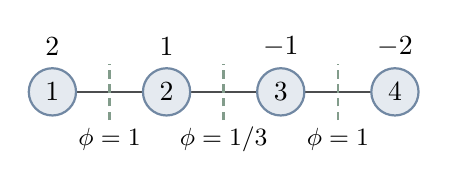
\begin{tikzpicture}[
  x=1.45cm,y=1cm,
  vertex/.style={circle,draw=graphSweepBlue,fill=graphSweepLight,
    line width=.8pt,minimum size=6mm,inner sep=0pt},
  cut/.style={draw=graphSweepGreen,densely dashed,line width=.85pt}
]
\definecolor{graphSweepBlue}{HTML}{7188A3}
\definecolor{graphSweepLight}{HTML}{E5EAF0}
\definecolor{graphSweepGreen}{HTML}{829C8B}
\definecolor{graphSweepLine}{HTML}{4C4D4F}
\draw[graphSweepLine,line width=.85pt] (0,0)--(3,0);
\foreach \i/\v/\f in {0/1/2,1/2/1,2/3/-1,3/4/-2}{
   \node[vertex] at (\i,0) {$\v$};
   \node at (\i,.57) {$\f$};
}
\foreach \i/\value in {.5/1,1.5/{1/3},2.5/1}{
   \draw[cut] (\i,-.36)--(\i,.35);
   \node[font=\small] at (\i,-.6) {$\phi=\value$};
}
\end{tikzpicture}

\caption{单位权四顶点路径上的阈值扫描。顶点上方标出了归一化谱方向还原后的函数值。三条竖虚线对应三个候选阈值，每个阈值恰好切过一条边。}
\label{fig:graph-cheeger-path-sweep}
\end{figure}

用四点路径验证。各点度为$(1,2,2,1)$。取$\bm f=(2,1,-1,-2)^\top$，计算
\[
\bm L\bm f=(1,1,-1,-1)^\top=\tfrac12\bm D\bm f,
\]
可知$\bm f$确实是归一化特征值$\mu_2=1/2$对应的方向。负值侧和正值侧的体积各为$3$，取中位数$\tau=0$后正部为$\bm g=(2,1,0,0)^\top$。

沿边能量为$(2-1)^2+(1-0)^2+(0-0)^2=2$，度加权平方和为$1\cdot4+2\cdot1=6$，能量商为$2/6=1/3<\mu_2$。

$g_i^2$的取值为$(4,1,0,0)$，产生两个非空阈值区间。图~\ref{fig:graph-cheeger-threshold-intervals}在同一条阈值轴上标出了顶点入选和边被切过的区间。

\begin{BookInlineFigure}
  \centering
  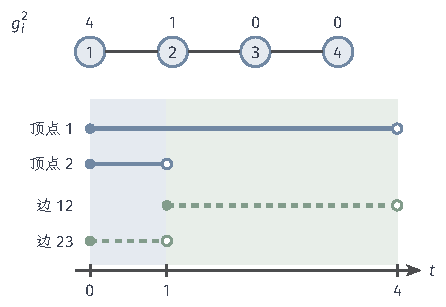
\includegraphics{figures/03-graphs/05-matrices-and-spectra/tikz/cheeger-threshold-intervals/figure.pdf}
  \caption{对$g_i^2=(4,1,0,0)_i$扫描阈值$t$。实线段标出顶点入选的区间，虚线段标出边跨割的区间。顶点$3,4$始终不入选，边$34$始终不被切过。}
  \label{fig:graph-cheeger-threshold-intervals}
\end{BookInlineFigure}

区间$[0,1)$选入$\{1,2\}$，体积$3$，割权$1$（边$23$被切），导通率$1/3$。区间$[1,4)$只选入$\{1\}$，体积$1$，割权$1$（边$12$被切），导通率$1$。

体积积分为$1\cdot3+3\cdot1=6$，割权积分为$1\cdot1+3\cdot1=4$。比值$4/6=2/3$，恰好位于两个导通率$1/3$和$1$之间。上界要求至少有一个候选不超过$\sqrt{2\cdot1/2}=1$，中间割的$1/3$远远满足。

直接按$\bm f$排序时，还有一个候选是$\{1,2,3\}$，它也只切过一条边，导通率为$1/3$。三个候选都只切一条边，中间位置的小侧体积最大，导通率最低。

\subsection{两端的紧性}
\label{sec:graph-cheeger-tightness}

Cheeger不等式的两端不能同时改进为同一个线性关系。下面通过两族图分别说明下界和上界各自的紧性。

\paragraph{下界取等：超立方体}

$d$维超立方体的$2^d$个顶点各有$d$条边，是$d$正则图。组合拉普拉斯的第二小特征值为$2$（沿任一坐标交替赋值$\pm1$给出这个值）。归一化后$\mu_2=2/d$。

沿某一坐标把顶点等分为两半。每个顶点恰有一条边跨割，每侧体积为$2^{d-1}\cdot d$。导通率为$2^{d-1}/(2^{d-1}\cdot d)=1/d$，恰好等于$\mu_2/2$。结合下界$\phi_*\geq\mu_2/2=1/d$，可以断定$\phi_*=1/d$。这说明下界的等号确实可以达到。

\paragraph{上界中的平方根尺度：长环}

对偶数$n\geq4$的环$C_n$，每个非平凡割至少切过两条边。取相邻的$n/2$个顶点为一侧，割权为$2$，该侧体积为$n/2\cdot 2=n$，导通率为$2/n$。可以验证这就是最小导通率$\phi_*=2/n$。

归一化拉普拉斯的第二小特征值为
\[
\mu_2=1-\cos(2\pi/n).
\]
当$n$增大时，$1-\cos(2\pi/n)\approx 2\pi^2/n^2$，因此$\mu_2$是$n^{-2}$阶的量，而$\phi_*=2/n$是$n^{-1}$阶的量。两者之间确实存在平方根的尺度差距：$\phi_*$与$\sqrt{\mu_2}$同阶。这说明上界$\phi_*\leq\sqrt{2\mu_2}$中的平方根不是证明技巧造成的损失，而是反映了长环这类图的真实结构。

这两族图放在一起看，下界可以精确取等，上界中的平方根指数不能改进。但两端并不在同一族图上同时取等——超立方体实现了下界的常数，长环展示了上界的指数。
